
\begin{TP}[Droite d'Euler]

\begin{enumerate}
\item Construis un triangle $DOC$ tel que $DO = 16$ cm, $OC = 12$ cm et $CD = 10$ cm.
\item Construis les hauteurs du triangle $DOC$ issues des sommets $D$, $O$ et $C$. Ces hauteurs sont concourantes. Nomme ce point d'intersection $H$ (ce point est l'orthocentre du triangle).
\item Trouve le centre $I$ du cercle circonscrit du triangle $DOC$.
\item Construis les trois médianes du triangle $DOC$. Ces médianes sont concourantes. Nomme ce point d'intersection $G$ (ce point est le centre de gravité du triangle).
\item Vérifie que les points $H$, $I$, $G$ sont alignés.

La droite qui passe par ces trois points est appelée la droite d'Euler. C'est le mathématicien Suisse Leonhard Euler (1707 - 1783) qui démontra en premier que ces points étaient alignés.
\end{enumerate}

\end{TP}

%%%%%%%%%%%%%%%%%%%%%%%%%%%%%%%%%%%%%%%%%%%%%%%%%%%%%%%%%%%%%%%%%%%%

\begin{TP}[Pavage par triangles curvilignes]

\partie{Un triangle curviligne}

\begin{enumerate}
 \item Réalisez la figure ci-dessous sachant qu'elle est composée d'un triangle équilatéral de 6 cm de côté et que le diamètre des disques est deux fois plus petits que la longueur d'un côté du triangle.
 \end{enumerate}
 
 \begin{center} 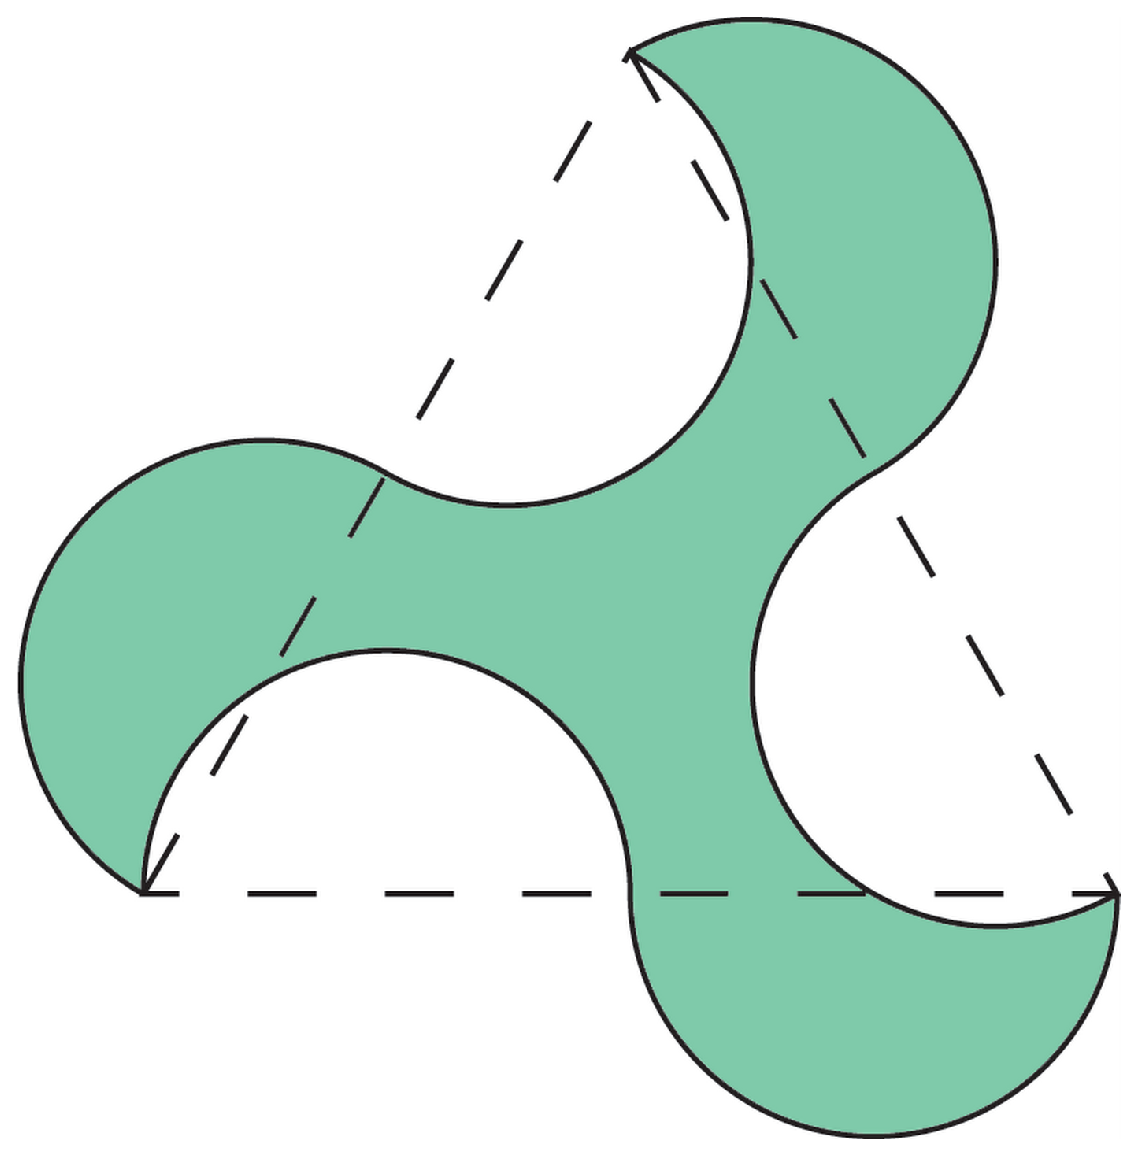
\includegraphics[width=3.5cm]{t_curviligne} \end{center}

\partie{Pavage du plan}

\begin{enumerate}
 \item Sur une feuille A4, réalise le maximum de triangles curvilignes en les plaçant les uns contre les autres. Coloriez les figures selon votre inspiration.
 \item En plaçant les triangles curvilignes les uns contre les autres, réalisez des frises décoratives et comparez vos résultats avec les autres réalisations.
 
 \begin{center} 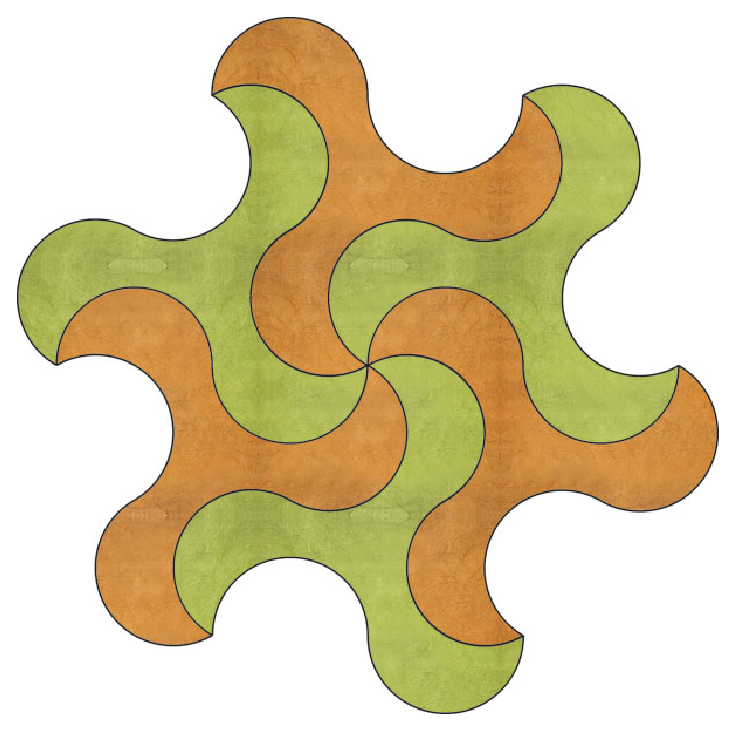
\includegraphics[width=3.5cm]{pavage} \end{center}

 \end{enumerate}

\end{TP}

